\section{Part III: Adaptive Learning}

\subsection{Choice of Adaptive Method}
In this work, the Adam optimizer~\cite{kingma2014adam} is selected due to its effective combination of momentum and adaptive learning rate methods. Adam computes individual step sizes for each parameter by maintaining exponential moving averages of both past gradients and squared gradients. This adaptation helps to handle sparse gradients and noisy data while ensuring fast convergence and robust performance. Notably, as reported by Tato and Nkambou~\cite{tato2018improving}, CNNs with Adam achieved a test accuracy of 99.12\% on the MNIST dataset, underscoring its practical benefits.

\subsection{Mathematical Formulation}
Adam's update mechanism is defined by the following equations:

\[
    m_t = \beta_1 m_{t-1} + (1 - \beta_1) g_t,
\]
\[
    v_t = \beta_2 v_{t-1} + (1 - \beta_2) g_t^2,
\]

where \(g_t\) is the gradient at time \(t\), and the decay rates for the first and second moment estimates are \(\beta_1 = 0.9\) and \(\beta_2 = 0.999\), respectively.

Bias-corrected estimates are computed as:

\[
    \hat{m}_t = \frac{m_t}{1 - \beta_1^t},
\]
\[
    \hat{v}_t = \frac{v_t}{1 - \beta_2^t}.
\]

The parameter update rule becomes:

\[
    w_{t+1} = w_t - \eta \frac{\hat{m}_t}{\sqrt{\hat{v}_t} + \epsilon},
\]

where \( \eta \) is the learning rate and \( \epsilon \) is a small constant to prevent division by zero. This framework enables Adam to adjust learning rates for each parameter adaptively, facilitating efficient convergence and improved performance.

\subsection{Results and Discussion}

\begin{figure}[ht]
    \centering
    % First sub-figure: Combined training plot (loss and accuracy over iterations)
    \begin{minipage}[t]{0.45\textwidth}
        \centering
        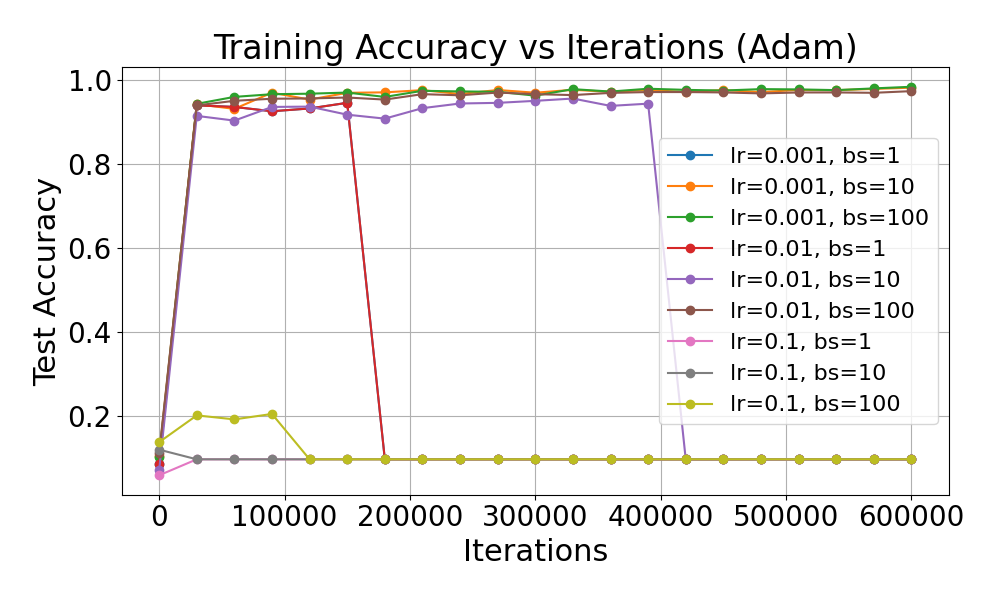
\includegraphics[width=\linewidth]{../data/part3/accuracy_training_plot}
        \caption{Accuracy across Iterations (Adam)}
        \label{fig:adam_combined_training_plot}
    \end{minipage}
    \hfill
    % Second sub-figure: Accuracy around the optima (>30000 iterations)
    \begin{minipage}[t]{0.45\textwidth}
        \centering
        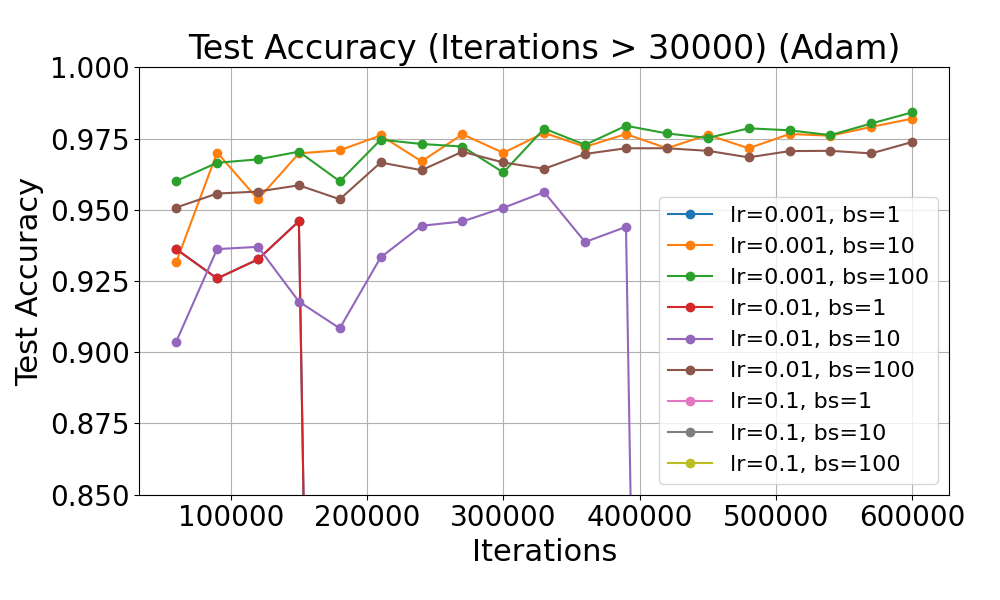
\includegraphics[width=\linewidth]{../data/part3/accuracy_training_plot_post_30000}
        \caption{Detailed Accuracy after 30000 Iterations (Adam)}
        \label{fig:adam_accuracy_after30000}
    \end{minipage}
    \hfill
\end{figure}

\begin{wraptable}{r}{0.38\textwidth}
    \centering
    \begin{tabular}{|c|c|c|c|}
        \hline
        \textbf{\(\eta\)} & \textbf{\(m\)} & \textbf{Loss} & \textbf{Accuracy} \\
        \hline
        0.01 & 100 & 0.0780 & 0.9738  \\
        0.001 & 10 & 0.0299 & 0.9820  \\
        0.001 & 100 & 0.0171 & 0.9842 \\
        \hline
    \end{tabular}
    \caption{Performance metrics at epoch 10 of the Adam optimizer.}
    \label{tab:adam_final_accuracy}
\end{wraptable}

The results of the Adam optimizer are presented in Figure~\ref{fig:adam_combined_training_plot}, \ref{fig:adam_accuracy_after30000}, and Table~\ref{tab:adam_final_accuracy}. From the figures, the configuration with a learning rate $\eta=0.01$ and a batch size $m=100$, as well as that with $\eta=0.001$ and $m=10$ or $100$, achieved convergence. However, these settings exhibited marked oscillatory behavior during training, suggesting that the adaptive updates still introduce significant fluctuations even when convergence is eventually attained.

In contrast, other parameter combinations using Adam either failed to converge or experienced collapse during the convergence process. This behavior highlights the sensitivity of Adam to hyperparameter choices, especially in scenarios involving small batch sizes or aggressive learning rates~\cite{li2024surge}.

When comparing with SGD, only the scenario with an large learning rate ($\eta=0.1$) combined with a small batch size ($m=1$), SGD failed to convergence. Overall, SGD demonstrated a higher degree of robustness under varied hyperparameter settings. And for the configuration with a batch size of 10, an initial learning rate of 0.1 decaying to a final learning rate of 0.0001, and a momentum coefficient of 0.1, SGD achieved the lowest loss of 0.0016 at epoch 10.

However, Adam's performance was superior in terms of final accuracy at epoch 10, as shown in Table~\ref{tab:adam_final_accuracy}. The best-performing configuration achieved an accuracy of 98.42\%, surpassing the best SGD configuration (98.28\%).

\section{Conclusion}
\paragraph{Limitations and Future Work}
This study identified several limitations for further investigation that could enhance performance and deepen understanding. Firstly, some experimental configurations did not fully converge within ten epochs; therefore, future work can consider extending the number of training epochs to determine whether these configurations eventually converge to superior results. Secondly, hyperparameter space are not fully explored, some hyperparameter optimization techniques like bayesian optimization~\cite{Frazier2018} may further improve model performance. Thirdly, given the observed benefits of learning rate decay, increasing batch sizes appears promising~\cite{smith2017dont}. Finally, the Nadam optimizer, which integrates Adam with Nesterov momentum, may yield enhanced performance~\cite{tato2018improving}.

\paragraph{Generalization to Other Problems}
Adam’s adaptive learning capabilities generalize effectively across domains beyond image classification. It is the optimizer of choice for natural language processing models like Transformer~\cite{vaswani2017attention}. It is also utilized in time series forecasting with LSTMs and GRUs~\cite{Makinde2024}. Furthermore, Adam is widely adopted in reinforcement learning algorithms, where its adaptive learning rates and momentum terms facilitate stable and efficient training of policy and value networks in dynamic environments~\cite{AsadiEtAl2023}.
